\documentclass[oneside,11pt,letter]{article}

% General include (DO NOT MODIFY)
\usepackage{amsmath,graphicx,cite,latexsym,color, amssymb,ifthen,verbatim}

\usepackage{listings}
\definecolor{mygreen}{rgb}{0,0.6,0}
\definecolor{mygray}{rgb}{0.5,0.5,0.5}
\definecolor{mymauve}{rgb}{0.58,0,0.82}

\lstset{ %
  backgroundcolor=\color{white},   % choose the background color
  basicstyle=\footnotesize,        % size of fonts used for the code
  breaklines=true,                 % automatic line breaking only at whitespace
  captionpos=b,                    % sets the caption-position to bottom
  commentstyle=\color{mygreen},    % comment style
  escapeinside={\%*}{*)},          % if you want to add LaTeX within your code
  keywordstyle=\color{blue},       % keyword style
  stringstyle=\color{mymauve},     % string literal style
}
\lstset{basicstyle=\small\ttfamily,breaklines=true}

%--------------- Various Style Declarations ----------------------------
\textheight 9in
\topmargin 0in
\headheight 0in
\headsep 0in
\textwidth 6.5in
\oddsidemargin 0in
\evensidemargin 0in
\footskip 0.2in
\parskip 5pt
\parindent 0pt
\topsep 2pt
\partopsep 0pt
\itemsep 0pt
\pagenumbering{arabic}

\definecolor{shade}{gray}{0.85}


\newcommand{\solpagesize}%
{\ifthenelse{\equal{\type}{solutions}}{
\textheight9in
\textwidth6.5in
\oddsidemargin0in
\evensidemargin0in
\topmargin-0.75in
\topskip0in
\footskip0.70in
\pagestyle{empty}
\parskip 5pt
\parindent 0pt
}{}}

\newcommand{\bookletskip}[1] %
{\ifthenelse{\equal{\type}{booklet}}{\vspace{#1 in}}
}

\newcommand{\bookletpage} %
{\ifthenelse{\equal{\type}{booklet}}{\newpage}{}
}

\newcommand{\inbooklet}[1]{\ifthenelse{\equal{\type}{booklet}}{{#1}}}


%%%%%%%%%%%%%%%%%%%%%%%%%%%%%%%%%%%%%%%
% Here are the new definitions of the commands \problem (for main
% text of problem), \problempart (for parts (a), (b) etc of the problem
% and \solution (for text of the solution).  The usage is as follows.
%
%    \begin{enumerate}
%    \problem{label}{main text of first problem}
%    \begin{enumerate}
%    \problempart{text of part(a) of first problem}
%
%    \solution{text of solution to part(a)}
%    \problempart{\text of part(b)}
%
%    \solution{text of solution to part (b)}
%
% ..... and so on for succeeding parts
%
%    \end{enumerate}
%
%    \problem{label}{main text of second problem}
%    \begin{enumerate}
%    \problempart{text of part(a)}
%
%    \solution{text of solution to part(a)}
%    \problempart{\text of part(b)}
%
%    \solution{text of solution to part (b)}
%    \end{enumerate}
%    ........ and so on for other problems
%    \end{enumerate}
%
% Please note that there needs to be a blank line separating
% a problempart command and the succeeding solution command;
% else the problem part and the solution are typeset as one
% paragraph when we are printing both the problem and its
% solution.  However, it is OK if a problempart follows a
% previous solution without an intervening blank line.  Some day I will
% waste some time figuring out a way around this problem

\newcommand{\problem}[2]%
{\item\label{#1}%
\ifthenelse{\(\equal{\type}{problems}\)\or\(\equal{\type}{both}\)}%
 {{\bf[#1]\\}#2}{{\bf[#1]}}}
 % The problem name always prints on the first line (in boldface
 % and inside square brackets.  The problem text prints on
 % succeeding lines if we are printing problems only, or problems
 % and solutions both

  \newcommand{\problempart}[1]%
{\item{\ifthenelse{\(\equal{\type}{problems}\)\or\(\equal{\type}{both}\)}%
 {#1}{}}}
 % The tag ((a), or (b) or (c) etc.) of the text of the part of the problem
 % prints in the margin, and is followed by the text of the problem beginning
 % on the same line if we are printing problems only or problems and
 % solutions both

 \newcommand{\solution}[1]%
{\ifthenelse{\equal{\type}{both}}{{\bf{Solution:\ }}{#1}}%
 {\ifthenelse{\(\equal{\type}{solutions}\)}%
 {#1}{}}}
 % This command does not generate a tag ((a), or (b) or (c) etc.)
 % for the text, but uses the tag generated by the previous 
 % problempart or examproblempart command.  If only the solutions 
 % are being printed, then the text
 % of the solution is printed beginning on the same line as the tag.
 % If both problems and solutions are being printed, then "Solution:"
 % is printed in boldface followed by the text of the solution.

  %%%%%%%%%%%%%%%%%%%%%%%%%%%%%%%%%%%%%%%%%
  
   \newcommand{\answer}[1]%
  {\ifthenelse{\equal{\type}{both}}{{\bf{Your answer:\ }}{#1}}%
  	{\ifthenelse{\(\equal{\type}{solutions}\)}%
  		{#1}{}}}
  % This command does not generate a tag ((a), or (b) or (c) etc.)
  % for the text, but uses the tag generated by the previous 
  % problempart or examproblempart command.  If only the solutions 
  % are being printed, then the text
  % of the solution is printed beginning on the same line as the tag.
  % If both problems and solutions are being printed, then "Solution:"
  % is printed in boldface followed by the text of the solution.
  
  %%%%%%%%%%%%%%%%%%%%%%%%%%%%%%%%%%%%%%%%%
  
  
 \newcommand{\examproblem}[2]%
{\item {\ifthenelse{\equal{\type}{solutions}}{}{{\bf [#1 points]} #2}}}
% The first argument is an integer specifying the number of points.  The
% first argument (followed by the word "points") is printed inside square
% brackets in boldface.  The second argument is the text of the problem
% itself.


\newcommand{\examproblempart}[1]%
{\item{\ifthenelse{\(\equal{\type}{problems}\)\or\(\equal{\type}{both}\)\or\(\equal{\type}{booklet}\)}%
 {#1}{}}}
 % The tag ((a), or (b) or (c) etc.) of the text of the part of the problem
 % prints in the margin, and is followed by the text of the problem beginning
 % on the same line if we are printing problems only or problems and
 % solutions both

%%%%%%%  ENTER SOME PROBLEM SET SPECIFIC STUFF HERE  %%%%



%%%%%%%%%%%%%%%%%%%%%%
%CHANGE
%.   to booklet to print the problems only
%
%    to both to print problems and solutions
%%%%%%%%%%%%%%%%%%%%%%

\newcommand{\type}{booklet}
% \newcommand{\type}{both}

% Custom adjustments (CHANGE THIS FILE FOR ADDITIONAL ADJUSTMENTS)
\newcommand{\cN}{{\cal N}}

\DeclareMathOperator*{\argmin}{\arg\!\min}
\newcommand{\norm}[1]{\left\lVert#1\right\rVert}

%************************************************************************
%                                                                       *
%            End of preamble and beginning of text.                     *
%                                                                       *
%************************************************************************

\begin{document}
%------------------------- Title Page ----------------------------------
\thispagestyle{empty}
\baselineskip2.5ex
{\bf University of Illinois}
\hfill
Spring 2018

{\Large
\begin{center}
{\sf CS\,446: Machine Learning}\\ Homework 9\\
\end{center}
}
{\large
\begin{center}
{\color{red}Due on Tuesday, April 3, 2018, 11:59 a.m. Central Time}
\end{center}
}

\ifthenelse{\equal{\type}{booklet}}{}{}

\begin{enumerate}

%%%%%%%%%%%%%%%%%%%%%%%%%%%%%%%%%%%%%%
%%%%%  BEGINNING OF PROBLEMS LIST

% !TEX root = exam.tex
\ifthenelse{\equal{\type}{booklet}}{
\newcommand{\GMMkMeansStudSolA}{
%%%%%%%%%%%%%%%%%%%%%%%%%%%%%%%%%%%%
%%
%%.   YOUR SOLUTION FOR PROBLEM A BELOW THIS COMMENT
%%
%%%%%%%%%%%%%%%%%%%%%%%%%%%%%%%%%%%%
\vspace{0cm}
K-Means is un-supervised method.

}

\newcommand{\GMMkMeansStudSolB}{
%%%%%%%%%%%%%%%%%%%%%%%%%%%%%%%%%%%%
%%
%%.   YOUR SOLUTION FOR PROBLEM A BELOW THIS COMMENT
%%
%%%%%%%%%%%%%%%%%%%%%%%%%%%%%%%%%%%%
\vspace{0cm}
$r_{ik} \in \{0,1 \}$ This will make any data point $x_{i}$ belong to or not belong to centroid $\mu_{k}$ 

}

\newcommand{\GMMkMeansStudSolC}{
%%%%%%%%%%%%%%%%%%%%%%%%%%%%%%%%%%%%
%%
%%.   YOUR SOLUTION FOR PROBLEM A BELOW THIS COMMENT
%%
%%%%%%%%%%%%%%%%%%%%%%%%%%%%%%%%%%%%
\vspace{0cm}
$r_{ik} \in [0,1]$ This will make each line of matrix $R$ a probability vector of data point $x_{i}$ 
}

\newcommand{\GMMkMeansStudSolD}{
%%%%%%%%%%%%%%%%%%%%%%%%%%%%%%%%%%%%
%%
%%.   YOUR SOLUTION FOR PROBLEM A BELOW THIS COMMENT
%%
%%%%%%%%%%%%%%%%%%%%%%%%%%%%%%%%%%%%
\vspace{0cm}
The number of clusters should be two because when number of clusters equals to two, it is the elbow of the plot.

}

\newcommand{\GMMkMeansStudSolE}{
%%%%%%%%%%%%%%%%%%%%%%%%%%%%%%%%%%%%
%%
%%.   YOUR SOLUTION FOR PROBLEM A BELOW THIS COMMENT
%%
%%%%%%%%%%%%%%%%%%%%%%%%%%%%%%%%%%%%
\vspace{0cm}
No. Assume the first two initial centers we initialize both on the outer circle but one is on the right, the other is on the left. After running K-Means algorithm, we will get two cluster which contains both inner and outer semi-circle respectively. It is not what we expected.

}

%\newcommand{\GMMkMeansStudSolF}{
%%%%%%%%%%%%%%%%%%%%%%%%%%%%%%%%%%%%%
%%%
%%%.   YOUR SOLUTION FOR PROBLEM A BELOW THIS COMMENT
%%%
%%%%%%%%%%%%%%%%%%%%%%%%%%%%%%%%%%%%%
%\vspace{12cm}
%}
 %The students have to fill this file to print the solution
}{
\input{GMMkMeans_OurSolution} %This file will not be provided to students since it contains the solution
}

% Problem Explanation:
% - first argument is the number of points
% - second argument is the title and the text
\examproblem{10}{K-Means\\}


%%%%%%%%%%%%%%%%%%%%%%%%%%%%%%%%%%%%%%
%%%%%  BEGINNING OF SUBPROBLEMS LIST

\begin{enumerate}

 % Subproblem description
\examproblempart{Mention if K-Means is a supervised or an un-supervised method.
 \\}

\bookletskip{0.0}   %in inches

% Solution box
 \framebox[14.7cm][l]{
 \begin{minipage}[b]{14.7cm}
 \inbooklet{Your answer: \GMMkMeansStudSolA}
  
 \solution{\GMMkMeansSolA}
 \end{minipage}
 }
 
  % Subproblem description
\examproblempart{Assume that you are trying to cluster data points $x_{i}$  for $ i \in \{1,2 \dots D\}$ into K clusters each with center $\mu_{k}$  where $ k \in \{1,2, \dots K \}$. The objective function for doing this clustering involves minimizig the euclidean distance between the points and the cluster centers. It is given by  \begin{equation*}
\min\limits_{\mu} \min\limits_{r}\sum\limits_{i \in D} \sum\limits_{k =1}^{K} \frac{1}{2} r_{ik} ||x_{i} -\mu_{k}||_{2}^{2} \\
 \end{equation*} \\ How do you ensure hard assignemnt of one data point to one and only one cluster at a given time? Note: By hard assignment we mean that your are 100 \% sure that a point either belongs or not belongs to a cluster.\\}

\bookletskip{0.0}   %in inches

% Solution box
 \framebox[14.7cm][l]{
 \begin{minipage}[b]{14.7cm}
 \inbooklet{Your answer: \GMMkMeansStudSolB}
  
 \solution{\GMMkMeansSolB }
 \end{minipage}
 }
 
% Subproblem description
\examproblempart{What changes must you do in your answer of part b, to make the hard assingment into a soft assignment? Note: By soft assignment we mean that your are  sure that a point either belongs or not belongs to a cluster with some probability.\\}

\bookletskip{0.0}   %in inches

% Solution box
 \framebox[14.7cm][l]{
 \begin{minipage}[b]{14.7cm}
 \inbooklet{Your answer: \GMMkMeansStudSolC}
  
 \solution{\GMMkMeansSolC}
 \end{minipage}
 }
 
 % Subproblem description
 \examproblempart{Looking at the following plot, what is the best choice for number of clusters?}
  \begin{center}
 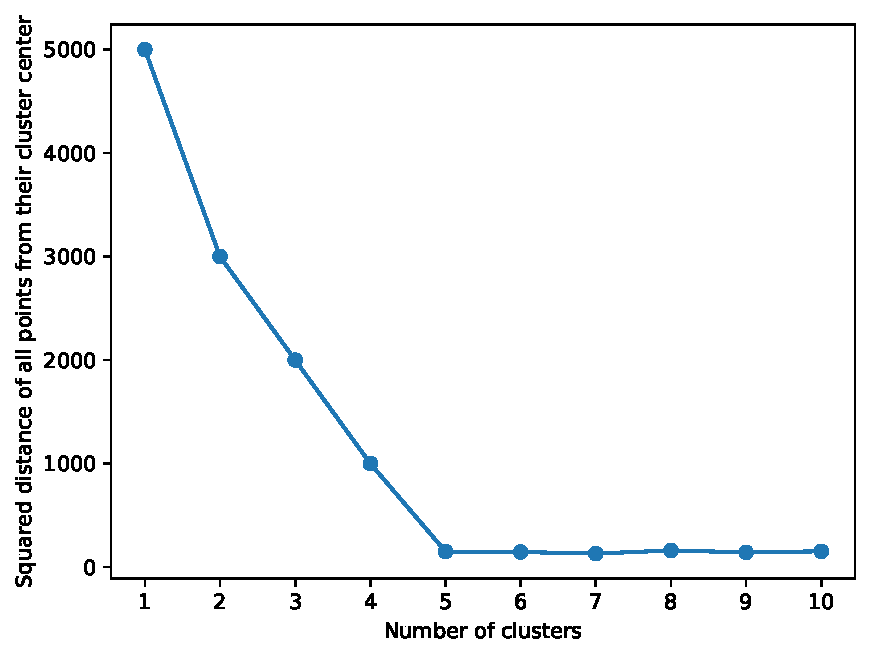
\includegraphics[width=8cm]{fig/cluster.pdf}
 \end{center}
\bookletskip{0.0}   %in inches

% Solution box
 \framebox[14.7cm][l]{
 \begin{minipage}[b]{14.7cm}
 \inbooklet{Your answer: \GMMkMeansStudSolD}
  
 \solution{\GMMkMeansSolD}
 \end{minipage}
 }

% Subproblem description
 \examproblempart{Would K-Means be an effecient algorithm to cluster the following data? Explain your answer in a couple of lines.}
  \begin{center}
 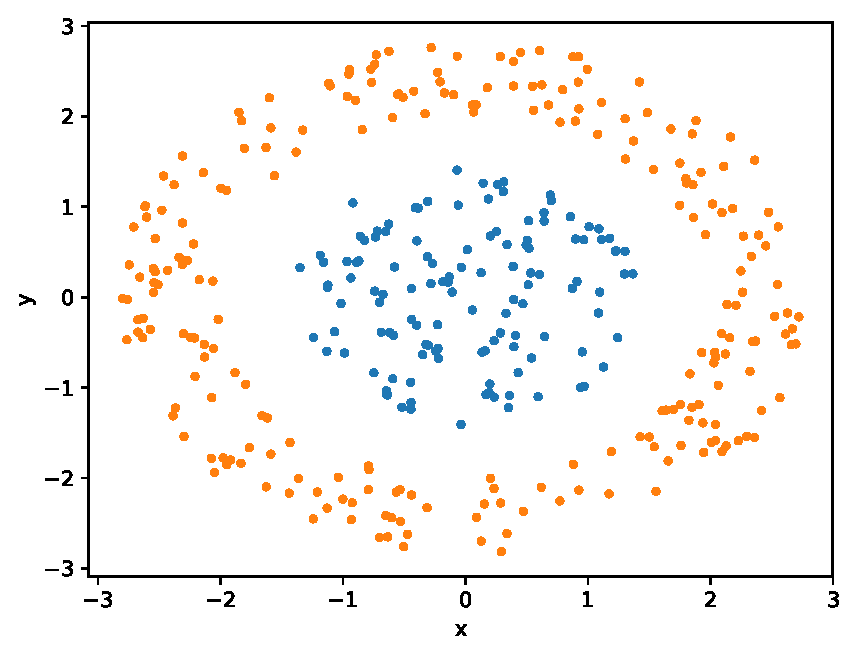
\includegraphics[width=8cm]{fig/concentric.pdf}
 \end{center}
\bookletskip{0.0}   %in inches

% Solution box
 \framebox[14.7cm][l]{
 \begin{minipage}[b]{14.7cm}
 \inbooklet{Your answer: \GMMkMeansStudSolE}
  
 \solution{\GMMkMeansSolE}
 \end{minipage}
 }
 
 %}
 
  %%%%%%%%%%%% END OF SUBPROBLEMS LIST
  
 \end{enumerate}
\bookletpage

%%%%%%%%%%%% END OF PROBLEMS LIST

\end{enumerate}
\end{document}
